\section{Simulations (Dave + Di Falco)}
\label{sec:simulation}

Prior to the start of operations, the main purpose of Mu2e simulation was to verify the expected performance of the experiment, and to allow optimization of the detector design. That required an accurate, detailed and flexible model of the experiment. In the analysis phase, the simulation will be used to optimize alignment, calibration, and reconstruction algorithms, and to estimate the expected detector acceptance and resolution.  The Mu2e simulation was designed to satisfy both these objectives.

The Mu2e simulation is based on Geant4 \cite{geant4:2003,geant4:2006,geant4:2016} and includes:
\begin{itemize}
\item a description of the {\em as built} geometry and the material composition for both the subdetector parts and the experimental hall,  
\item the temporal and spatial structure of the proton beam,
\item magnetic field maps,
\item the treatment of the physics processes which particles undergo while passing through the experimental apparatus,
\item a set of custom event generators dedicated to the conversion electron channel and the main sources of background, 
\item the implementation of the detector response as measured at beam tests and with cosmic rays, 
\item the interface with the calibration database, 
\item the full event simulation including the overlap with the beam background particles.
\end{itemize}
Several simulation campaigns have been conducted to optimize the detector design and study the experimental sensitivity to the muon conversion.
Additional studies have been performed using other Monte Carlo codes (MARS\cite{MARS:2009}, MCNP\cite{MARS:2009,MCNP:2012}, FLUKA\cite{FLUKA:2013}, PHITS\cite{PHITS:2018}) to validate Geant4 predictions and to estimate their uncertainty.

\subsection{ Geometry description}

\begin{figure}[htb]
\begin{center}
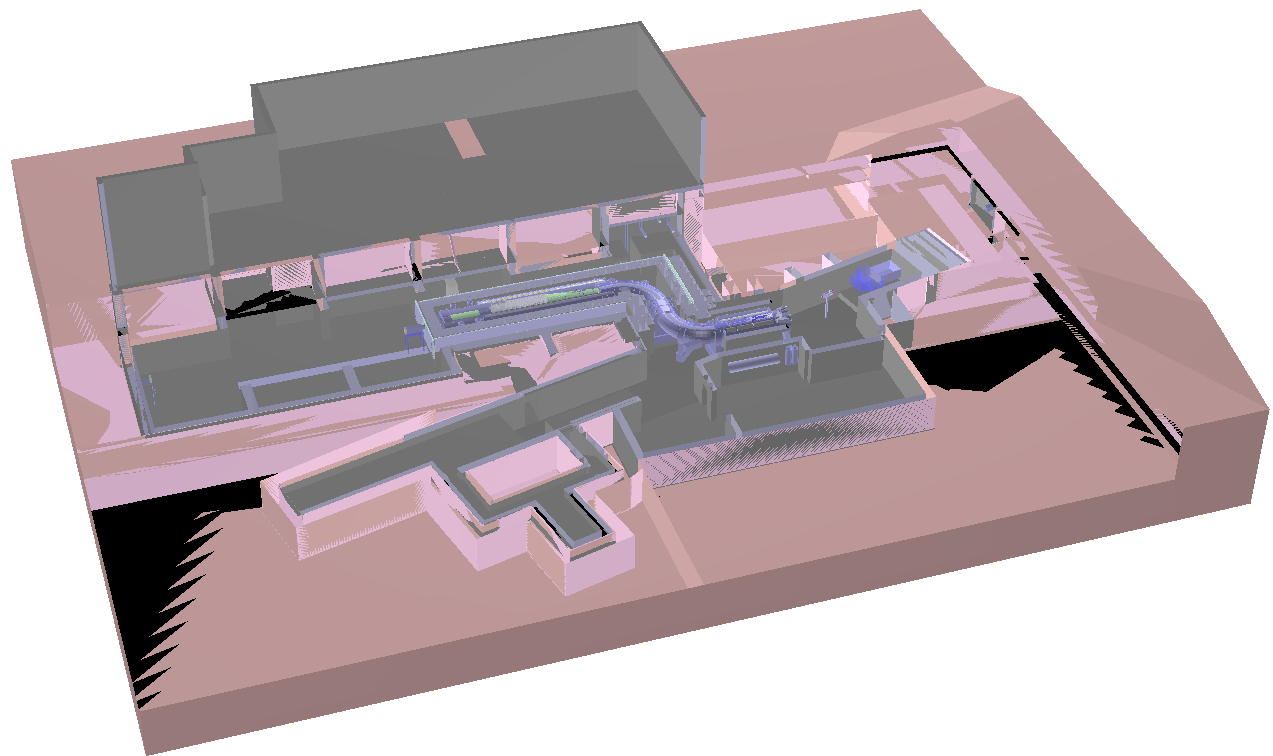
\includegraphics[height=0.29\linewidth]{figures/mu2eHall.png}
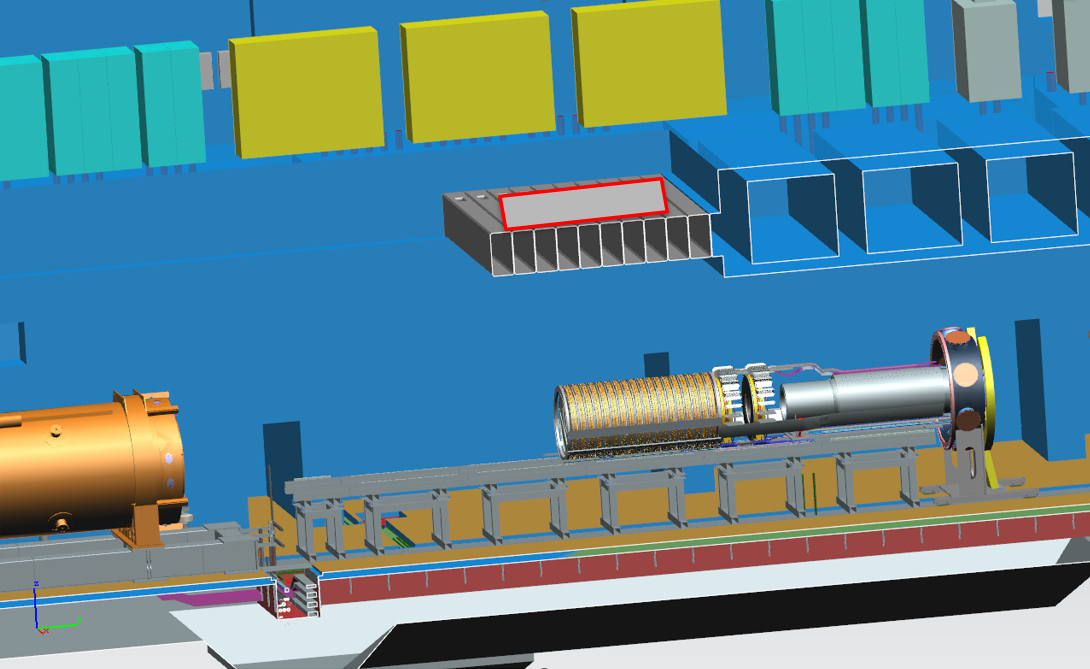
\includegraphics[height=0.29\linewidth]{figures/geom_extracted.png}
\caption{Left: the Mu2e experiment and building in the Geant4 Offline simulation. Right: Mu2e detectors in the extracted position.}
\label{fig:mu2e_geom}
\end{center}
\end{figure}

The picture on the left of Figure~\ref{fig:mu2e_geom} shows the image of the experimental hall as designed for the first run of the experiment: it is realized using the Geant4 geometry routines to create the logical and physical volumes and check for their overlaps, to assign the material composition to both active and passive volumes, to define virtual detectors to study particle fluxes and to graphically display the result.

For the passive part the relevant information obtained from the simulation is the effectiveness of the shielding against the radiation produced by beam interactions and cosmic rays. The simulation includes the dirt surrounding the detector hall, the building walls, the concrete shielding blocks, the solenoids warm and cold mass including the individual coils, the heat and radiation shield, the  production target with its support, the beam collimators, the antiproton absorbers, the stopping target with its support, the inner and outer proton absorbers, the mechanical structure of tracker and calorimeter including electronics and cables, the beam dump downstream of the proton beam with the extinction monitor, the beam dump downstream of the muon beam, the stopping target monitor outside of the DS.
The amount, type and location of shielding has been decided as a compromise between budget considerations and the amount of radiation acceptable for the different subdetectors and the magnetic coils. It will be reviewed for Run II according to the result of Run I.
 
The geometrical description of each subdetector is maintained by the corresponding working groups, coordinated by the Simulation group. One or more geometry files exist for each subdetector to ensure a sufficient degree of modularity. The level of detail of the geometry description is a compromise between the time needed to simulate the events and the agreement between data and Monte Carlo simulation.

The main parameters of each subdetector such as material composition, number of elements, single element dimension and location, are included in the geometry database. \red {[at the moment we still have some text file: do we want to specify this?]}. Also the sensors and electronic boards located inside the detector solenoid have been simulated in detail to study the radiation levels expected for each of them.  

The dimensions and positions of the active parts (TRACKER straw tubes, ECAL crystals, CRV scintillators, STM crystal and strips, EXTM pixel pads)  are the nominal ones: mechanical tolerances, gravitational sags or misalignments are introduced at the digitization level.

A separate geometry package has been realized for the detector commissioning with cosmic rays.  The simulation of the experimental setup  in this so called {\em extracted position} includes the tracker and calorimeter out of the Detector Solenoid and few modules of the Cosmic Ray Veto on top of them (Figure~\ref{fig:mu2e_geom}(right)).

Alternative geometrical descriptions for the detector have been realized using MARS and FLUKA to determine the uncertainty of simulation estimates of the radiation levels and the stopped muon yield.

Each subdetector group has developed the geometry description of the setup used for beam or cosmic ray tests of the prototypes or for the Vertical Slice Test of the first production modules. Although these are in general standalone programs, they have been an important tool to validate the detector description in the Offline repository.  

\subsection{ Magnetic field maps}

Detailed magnetic field maps are produced using the OPERA 3D \cite{opera3D} and HELICALC \cite{helicalc}  software packages using (warm) as-measured conductor geometries and coil positions provided by the Mu2e project solenoid construction team.  The field is stored as a discrete vector map over a Cartesian grid, separately for the Production Solenoid (PS), Transport Solenoid (TS), Detector Solenoid (DS), and the region outside all the solenoids.  The effect of re-bar in the concrete shielding has been calculated but not yet included.  Field maps for special run conditions used for calibration purposes have also been generated. The field map is accessed through a software interface that dynamically interpolates the field vectors from the 9 grid points nearest the requested reference point.

The Mu2e operations team will determine the in-situ DS magnetic field using a custom survey device that will measure the magnetic field components at fixed locations within a cylindrical coordinate grid.  A fit to the measured data using a combination of a multi-pole expansion and relaxation ANN constrained to Maxwell's equations will be used to interpolate and average the measurements into the Cartesian grid format.  This map will be corrected for the estimated effect of re-bar in shielding materials that can't be in place during the field survey.

Due to operational constraints the field survey may not be performed until after run 1, in which case preliminary simulations and reconstruction will be performed using the estimated map. Publication quality simulations and reconstruction will use the field map determined from the survey. Changes in physics objects reconstructed using alternative maps spanning the measurement and shielding magnetization uncertainties will be used to estimate the systematic errors on physics measurements due to residual field map uncertainties.

\subsection{ Simulation of Physics processes}
\subsubsection{ Geant4}

The main physics interactions are simulated using a modification of GEANT4 "Shielding" physics list.  The main modification consists in increasing the threshold used to pass from the Bertini Cascade (BERT) model for low energy hadron-nucleus interactions to the Fritiof (FTF) model from 4-5 GeV to 9.5-9.9 GeV to better reproduce the experimental data on pion production.  

Nuclear de-excitations and radioactive decay of long-lived isotopes are included. 
Hyperon and anti-baryon production is obtained from the chiral invariant phase space model (CHIPS).

Neutron simulation uses the high precision model (HP) up to 20 MeV. This is particularly relevant for the prediction of the thermal neutron background.

For what concerns the processes related to the muon capture in the aluminum stopping target, Geant4 is used only to produce the electrons and the photons from the atomic cascade to the ground state. The nuclear muon capture, the muon decay in orbit, the radiative muon capture and the muon conversion are simulated using custom generators. The same holds for the radiative pion capture in the stopping target. 

Simulation of muon and pion captures outside of the stopping target is generally managed by Geant4. Custom generators have been created for particular studies concerning detector calibration like muon decay in orbit in the Inner Proton Absorber (IPA) or Radiative Muon Captures (RMC) in the gold-tungsten support wires of the stopping target.   

\subsubsection{ Other MC codes}

When no experimental data are available it's hard to infer the systematic error on the prediction obtained using a single Monte Carlo code.

For this reason other Monte Carlo codes have been used to validate and eventually correct Geant4 based estimates of some critical quantities.

MARS has been extensively used to study the radiation levels in the Mu2e hall, the effectiveness of the concrete shielding and of the Heat and Radiation Shield surrounding the PT, the dose and neutron fluence on tracker and calorimeter electronics.

The effect of concrete shielding on neutron and kaon radiation has been studied also with FLUKA and MCNP.
 
Pion production in the PT has been studied also with MARS, MCNP, FLUKA and PHITS.
  
Geant4 expectation for antiproton production in the PT in the backward direction has been corrected given its disagreement with MARS, MCNP and FLUKA\cite{SU2020:2023}. 


\subsection{ Simulation workflow}

The simulation of the large number of events expected in Mu2e requires some optimization of the processing time.
This is done using a staged simulation approach together with resampling techniques.

Given the statistical nature of the particle interactions in the material crossed before reaching the detectors, it's possible, where appropriate, to reuse many times the particles stored at the end of one stage ({\em resampling}) increasing the available statistics at a reduced cost of CPU time. The absence of statistical biases ({\em oversampling}) must be checked case by case.

The staged approach helps to save additional CPU time when no changes occur in the first stages and it's sufficient to rerun only the last stages. In addition, different particle range cuts can be used in the different stages avoiding a too much accurate and time expensive particle tracing when it's not needed.  

The main beam simulation is divided in four stages:
\begin{enumerate}
\item from the 8 GeV proton beam on the Production Target (PT) to the entrance of the Detector Solenoid (DS);
\item from DS entrance to the stopping target (ST);
\item from the ST to the exit from the DS volume (tracker, calorimeter and cosmic ray veto hits are stored);
\item hits digitization.
\end{enumerate}

The initial beam protons are given the nominal beam energy and direction, distributed across the PS entrance as a symmetric Gaussian with the width expected from beam simulations.  The time of each proton is sampled from a distribution generated by detailed simulations of the slow extraction and active extinction system. Target interactions are modeled using a physics list that includes the most up-to-date description of anti-proton production, among other things \red{more tosay here??  should we consolidate our description of physics lists?}.
To save processing time, charged particles which exit the PS volume going forwards are killed.

\subsection{Special Configurations}
To increase the statistics of pions stopped in the ST, their decay can be disabled. The stopped pion probability will then be corrected for the pion survival probability depending on its lifetime.     

For the antiproton simulation the first stage has been divided in four phases: interaction of the proton beam with the PT, generation of antiprotons from the inelastic vertices in the PT, tracing of antiprotons from the PT to the middle of the Transport Solenoid (TS) and finally to the DS entrance. The first two phases are needed to use a customized differential cross section for the antiproton production. The last two phases have been used to optimize the absorber window located at the center of TS. 

Also cosmic ray simulation requires a dedicated workflow. In the first stage secondaries produced  by CRY generator [reference] according to the flux at sea level are traced from the top of Mu2e building to the DS. Events are divided in three categories according to the energy deposited in the Cosmic Ray Veto (CRV): high (E>16 MeV), low (E<16 MeV) or null (neutrons or particles passing through the TS hole). In the following stage particles are resampled and traced through the detector. Finally digitization is performed.

In any case, to save disk space and computation time, only the events with a minimum energy deposit in the tracker, the calorimeter or the cosmic ray veto are passed to the digitization stage.


\subsection{ Custom event generators}

A set of generators have been realized to have a more accurate simulation of the particle yield from the stopping target. Starting from the position and time of the stopped muons or pions and reusing them many times {\em resampling}, the following single particles can be generated with isotropic direction: conversion electron (Leading Log spectrum from  ~\cite{Czarnecki:2011mx,Szafron:2017guu}),  conversion positron (Leading Log spectrum from  ~\cite{Czarnecki:2011mx,Szafron:2017guu} rescaled to the expected peak momentum of  92.3 MeV/c), DIO (Leading Log spectrum from ~\cite{Szafron:2016}), muon capture secondaries (protons and deuterons spectrum adapted from \cite{TWIST:2020,ALCAP:2022}, neutron spectrum is adapted from Ca measurements ~\cite{MCnspectrum:1978} and normalized according to ~\cite{MCnnorm:1965}, X and gamma rays used to study the Stopping Monitor response are generated as single lines), radiative muon capture secondaries (photon spectrum from the fit of experimental data \cite{TRIUMF:1999} with the closure approximation \cite{closureapprox}, resampling of photon conversions, e+e- pairs from Geant4 Bethe Heitler cross section implementation), radiative pion capture secondaries  (photon spectrum adapted from Mg data ~\cite{Bistirlich:1972}, resampling of photon conversions, e+e- pairs from Geant4 Bethe Heitler implementation).

Cosmic ray studies for the Mu2e TDR\cite{TDR} have been performed with the Daya Bay generator\cite{DayaBay} and checked with CRY generator\cite{CRY:2007}. A recent evaluation of CE sensitivity  for Mu2e Run I has used the CRY generator to evaluate the cosmic background and the CORSIKA generator ~\cite{CORSIKA:1998} to evaluate the uncertainty on flux normalization.  

A custom generator to produce antiprotons from protons interaction in the PT has been developed fitting the existing data and extrapolating them to the 8 GeV Mu2e beam energy \cite{SU2020:2023}.


\subsection{ Simulation of detector response}
Each subdetector has a dedicated simulation of its digitization. This includes a parameterization of the physics processes bringing the signal from the position where the energy is deposited to the readout electronics and also the simuation of the electronics response. \red {So we foresee to use some database information during digitization?}
\begin{itemize}
\item{Tracker}
 \red {to be checked with Dave or Richie}

Energy deposits in the straw tubes are processed through applying a parameterized simulation of the drift time (incuding gravitational sag \red {is it true?}), gas amplification, signal transit time along the wire, electronic amplification and shaping. Electronic signals at the straw ends are superimposed and the resultant waveform is digitized. Only digitized hits passing the discrimination threshold are saved.
\item{Calorimeter}
 \red { to be checked with Bertrand}

  Energy deposits in each crystal are grouped in time. The number of photons produced by scintillation takes into account the avearge light response uniformity measured during crystals qualification. The number of photoelectrons obtained using the average PDE of the SiPMs is smeared with a Poisson distribution. The digitizer waveforms corresponding to energy deposits in the same readout unit are superimposed. Radiation induced noise and electronic noise is added. Zero suppression is reproduced.
\item{Cosmic Ray Veto}
\red { to be checked with Ralph or Yuri}

Energy deposits in each module are grouped in time. The bunch time structure is applied (only for the on-spill simulation). The time distribution of the charge collected by the SiPMs located at the edge of each module is calculated using the scintillator light yield, the WLS collection efficiency, the light attenuation along the fiber, the reflection probability on the walls and the SiPM photon detection efficiency \red {database information?}. The charge collected by the SiPMs is tranformed in signal waveforms after applying a random time jitter and photoelectron fluctuation. ADC and TDC counts are obtained applying waveform sampling and discrimination. 

\item{Stopping Target Monitor}
\red { HPGe checked with Pawel, waiting for inputs on LaBr}

The energy deposited by each photon in the HPGe detector is used to generate a waveform according to the deposited ionizing energy, measured gain, and collection efficiency. Waveforms from different photons are superimposed using the expected time and energy distribution. Electronic noise from the pre-amplifier and amplifier is added. The resulting waveforms are digitized using the 16bit ADC, and are used together to form STMWaveformDigis. A similar technique will be used for LaBr response.

\item{Extinction Monitor}
\red { checked with Andrei}

Energy deposits are converted into electron-hole pairs. Number of charge carriers is fluctuated 
using the silicon Fano factor of 0.1. Deposited charge is split in a number of clusters uniformly distributed along the particle path inside the sensor. Each cluster is drifted individually. The sum of the charge reaching the preamplifier with its time structure is passed to a discriminator that simulates the time and time over threshold response of the readout chip. At the final stage the digitization algorithm adds random hits to the output \cite{ExtMon:2014}.

\end{itemize}

\subsection{ Pileup simulation}
In addition to signal particles of interest for physics, Mu2e must model the \emph{pileup} of many low energy particles produced by beam particles and decay/capture products of the vast majority of stopped muons which do not convert to electrons, or produce a particle which could be a signal background, as described above. 
Pileup is not itself a source of backgrounds for physics analyses, but the detector signals it generates can significantly affect the reconstruction efficiency and/or resolution of signal and signal-like particles.

Mu2e currently simulates pileup using Geant-4, starting with protons hitting the production target (POT), as described above. Charged particles which travel backwards and enter the TS are check-pointed as they enter the DS. Neutral particles that exit the beamline are check-pointed as they exit the TS or PS volume.

In subsequent simulation jobs, each check-pointed particle's passage through the DS is resampled  1000 to 10000 times, depending on the sample. Particles which produce energy deposits in detector sensitive volume are saved, along with their genealogy and energy deposits. To allow correct normalization when used downstream, the fraction of saved events is calculated automatically during the resampling, relative to the original number of simulated POT, and stored in the conditions database.

Resampled muons which stop in the stopping target are check-pointed before they decay, and then resampled 10000 times in-turn to model pileup from muon capture and decay daughters. The muon lifetime is randomly sampled each resampling, and custom codes are used to randomly select a ddecal  or capture decay mode. These same check-pointed
target-stopped muons are also used as starting space-points in the signal generators described above. The efficiency of resampled stopped muons to produce detector sensitive volume energy deposits is computed and recorded in the database.

Pileup in the CRV is dominated by the neutral particles (mostly neutrons) leaving the PS.  As the cross-section for generating signals in the CRV are small, these can be resampled many times, currently 10000. A physics list including detailed neutron interactions is used for this stage.  Neutral CRV pileup resampling dominates the resources needed for pileup simulation, as the required statistics are large and the processes involved are time-consuming to model.

Pileup is overlaid on signal events by adding the sensitive volume energy deposits from an appropriate number of pileup daughters to the energy deposits generated by the signal process particle. Pileup data are read through art secondary input streams, in sequential mode, starting from a random starting event.
The number of pileup daughters needed is computed for each event by sampling the expected POT distribution, scaling that by the products of the relevant resampling efficiencies read from the database, and then applying Poisson fluctuations.  The resulting summed energy deposits are then passed through the detector response simulation. Since proton pulse intensity is almost constant on the time scale of few $\mu $s (few proton pulses), and the pulse trains are long, the time of each pileup particle energy deposit is wrapped around the 1.695 $\mu s$ bunch period when summing.

Most Mu2e pileup simulations use a POT intensity distribution modeled by a log-normal distribution with Spill Duty Factor (SDF) = 60\%~\cite{SU2020:2023}, scaled to the average beam intensity expected for operations with either 1 or 2 booster batches. A time-sequence of POT computed using a detailed beam extraction simulation can also be used.

Even with the efficiency scaling provided by resampling, simulating pileup starting from POT is very inefficient.  Using $\sim 10M$ core-hours of processing time, the most recent simulation campaign produced less than 1 second of actual beam time, and statistical artifacts due to over-sampling of some particles are evident in these samples.

To avoid the limitations of the Geant-4 based pileup simulation, Mu2e is developing code to overlay pileup extracted from data on simulated signals. By triggering randomly, Mu2e can record unlimited pileup events with essentially zero resource cost that will naturally track the real POT intensity, and follow changing detector conditions. Unlike with Geant-4, pileup recorded from data will be already digitized. Digital pileup data in channels that don't overlap with simulated signal particle energy deposits in time or channel can be used directly. 
Digital pileup that overlaps with simulated signal particle energy deposits in both time and channel must be reverse-digitized before merging, to allow analog-summing its effect before re-digitizing. For the tracker, 98\% of pileup signals are non-overlapping. Preliminary studies using simulated pileup show that digital overlay produces nearly identical results as energy-deposit overlay. Digital pileup overlay is currently only implemented for the tracker, and will be expanded to the calorimeter and CRV in the near future.

\subsection{ Simulation Interface with databases}
\red {already covered in database section?} 



\subsection{Monte Carlo Production (Sophie +)}
%\textcolor{red}{this can be moved elsewhere}

Large scale Monte Carlo Production is carried out by the Production Manager. In the Mu2e GitHub organization all relevant production scripts are stored in the Production repository: \url{https://github.com/Mu2e/Production}.

\subsubsection{MDC2020 Production (Sophie +)}

The MDC2020 campaign was a large scale production development campaign which built the foundations of our present Monte Carlo production infrastructure. MDC2020 relied heavily on the Production Operations Management Service (POMS) \cite{Mengel:2020wev} which is a soon to be discontinued CSAID tool that helped users to run large and complex grid campaigns. The major goals of MDC2020 were:
\begin{itemize}
    \item to improve the simulation realism and accuracy through using updated Geant4 version and detector geometry and informed detector response modeling;
    \item to develop and test infrastructure needed for commissioning and early data taking and analysis (calibration, misalignments…);
    \item produce samples needed for continuing algorithm development and analysis (trigger, alignment, calibration, monitoring, reconstruction, PID…).
\end{itemize}

The simulation starts by simulating protons hitting the production target (POT).  Currently the protons are modeled as a monochromatic beam directed at the target face center with no angular divergence and a Gaussian transverse spread, with sigma set by accelerator studies. The Geant4 is configured with a relative long minrange cut to speed the simulation. This simulation is stopped when the particles exit the TS.

The secondary simulation particles produced by the standard beam campaign are filtered and sorted into two output collections; beam and neutrals. Charged particles that reach the entrance of the DS are stored in the ‘beam’ collection.  Neutral particles that enter the DS, or any kind of particle that exits through the TS sides (almost fully neutral), are stored in the ‘neutrals’ collection.  The ‘beam’ collection is further split into muons (positive and negative), and other charged particles (almost exclusively electrons).  The muons collections are used for modeling signal processes and muon-induced pileup.  The electrons are used to model beam flash backgrounds. The neutrals collection is used to model pileup in the CRV and other detectors.  The muons stopped in the stopping target can be resampled many times, since the daughter production processes that follow are very random in terms of particles produced, particle momentum, decay time, etc.  An analogous pion beam campaign allows for production of RPC background samples.

In theory, large beam campaigns are ran only once (until there is a significant change in the simulation). These can then be used as input to many primary campaigns. Pile-up is mixed in on-top of the primary simulations to produced realistic samples for physics studies.

Another important aspect of MDC2020 was the consideration of different calibration and alignment conditions and the first to extract assumed parameters from the conditions data-base. Simulation efficiencies are also now extracted directly from the data-base. This allows prototyping of the conditions data-base within reconstruction, an important step in preparing for real-data reconstruction.


\subsubsection{Production Moving Forward (Ray should probably write this)}


\subsubsection{Mock Data Production (Sophie)}
\label{mock_data}

The purpose of Mock Data is two-fold: \begin{enumerate}
    \item they can be used to develop analysis tools and strategies;
    \item they can help us understand our data-production needs. 
\end{enumerate}

Mock Data is developed using a set of primary outputs from large-scale production. Each primary represents a given physics process (e.g. Cosmics, DIO, RPC etc.). Conversion signals (of a given conversion branching rate) are combined with decay-in-orbit (DIO) tail backgrounds (reaching below the trigger threshold to 75 MeV/c), cosmic backgrounds (from either the CRY or CORSIKA generator), radiative pion and muon capture backgrounds and pile-up. For this to be done accurately we must make assumptions about the incoming beam (how many protons per second), the livetime and the signal rate.

The combined sample is then passed through our digitization and reconstruction framework to create ``data-like" samples. Figure~\ref{fig:mockdata} illustrates the simulation stages needed to produce the Mock Data.

 \begin{figure}[htb]
\begin{center}
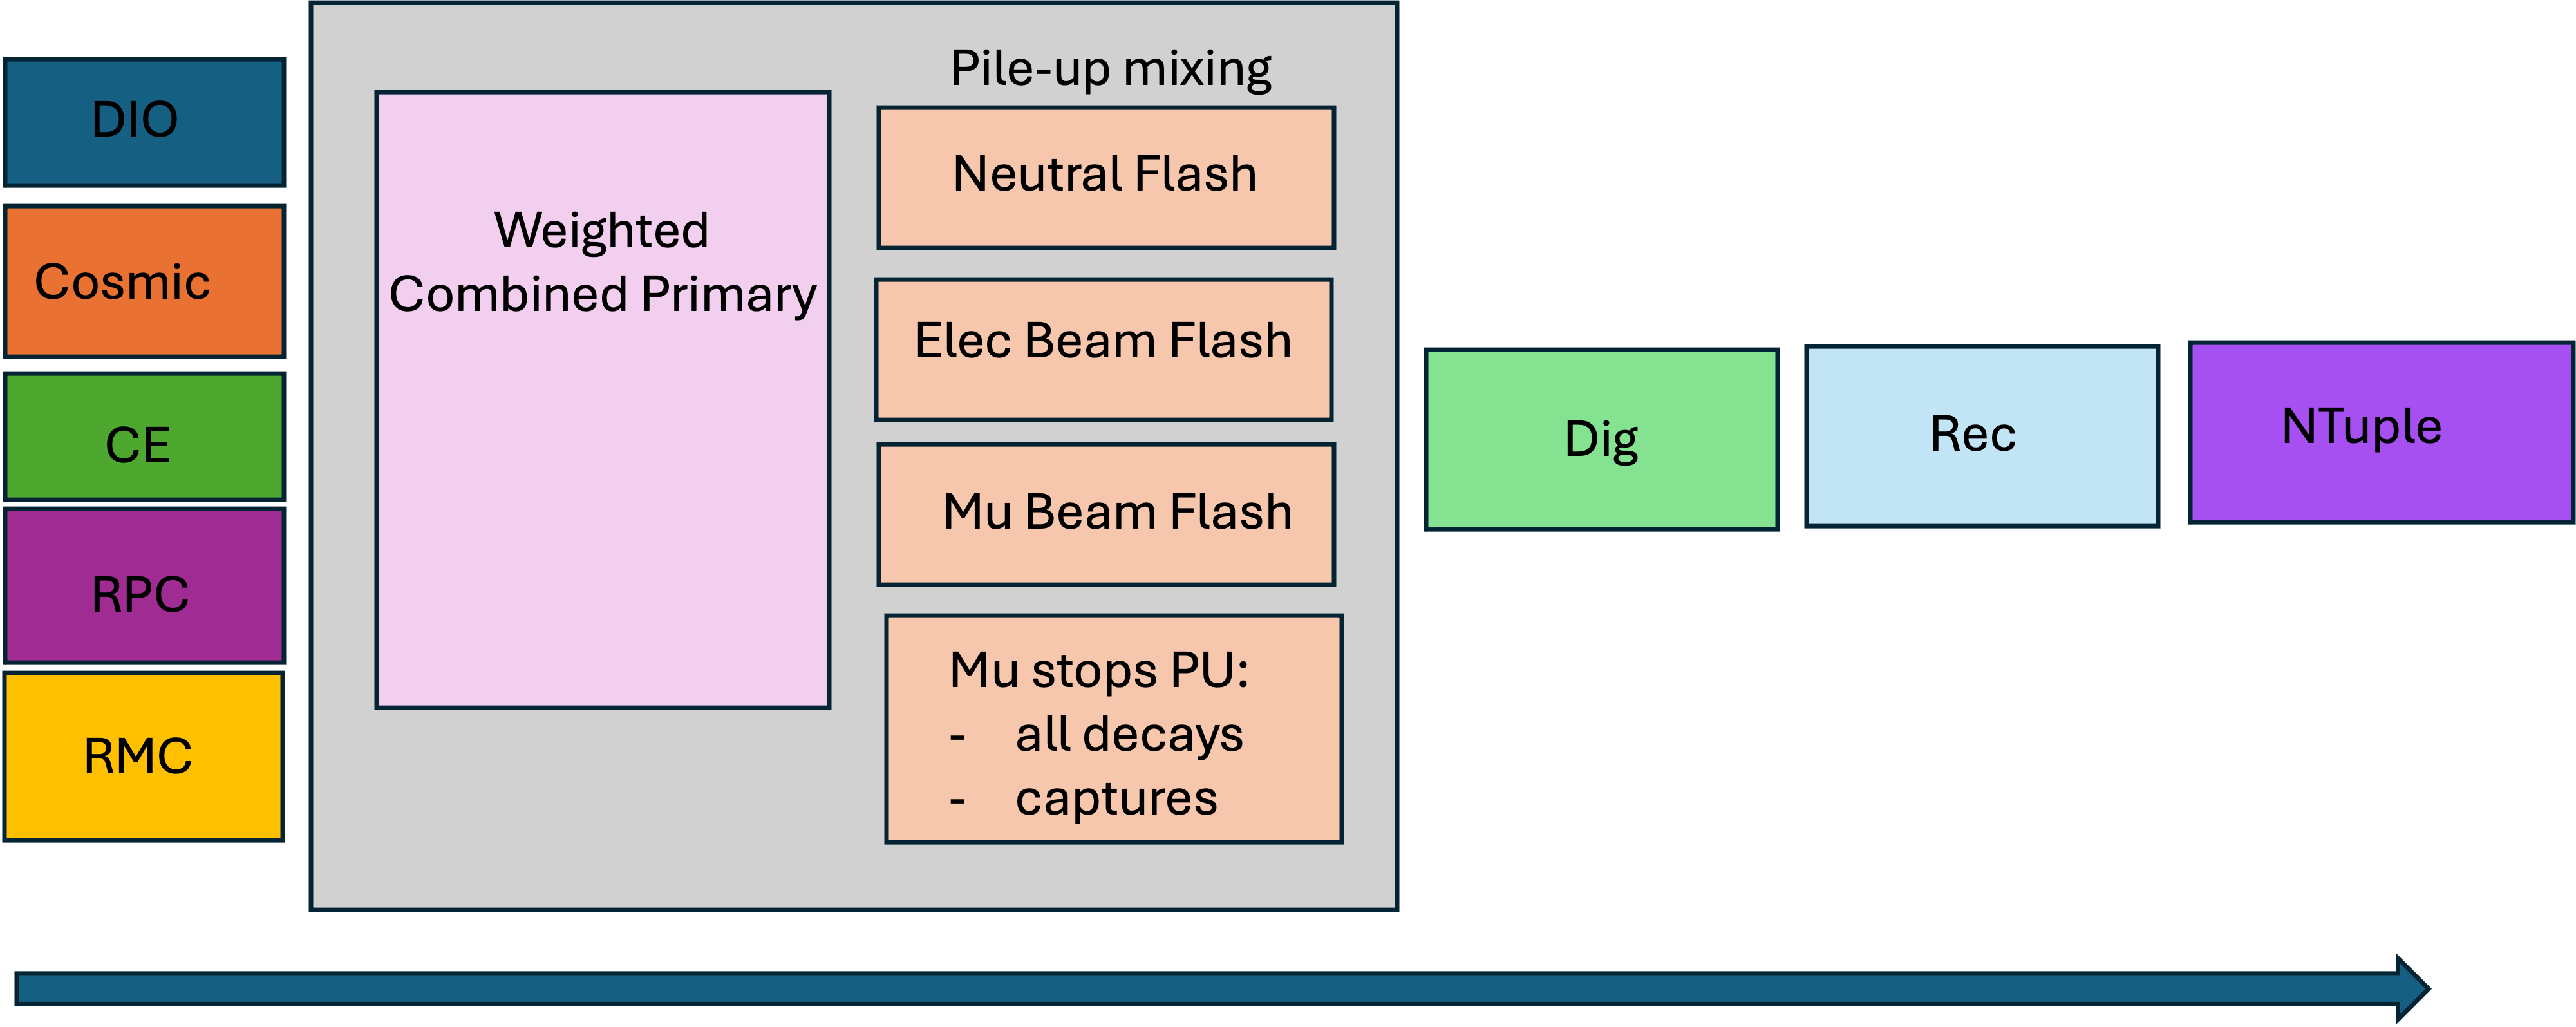
\includegraphics[width=0.7\linewidth]{figures/ensemblesMD0.png}
\caption{Illustration of how the Mock Data samples are created. Individual  production primaries (decay-in-oribt (DIO), conversion electron (CE), Radiative Pion Capture (RPC), Radiative Muon Campture (RMC) and cosmics are combined in weighted ratios (with knowledge of expected number of events for the chosen livetime). This combined set of events is then passed through the standard digitization and reconstruction workflows. The final output is an ntuple (currently TrkAna) which is input into the Reference Analysis.}
\label{fig:mockdata}
\end{center}
\end{figure}


\subsection{ Brief summary of previous simulation campaigns}

\begin{itemize}
\item {\bf CD3 studies}

\red {Do we want it?}

\item {\bf 2018 Mock Data Challenge (MDC2018)}
\red {Do we want it?}

\item {\bf 2020 Sensitivity Update (SU2020)}
An extensive simulation campaign with updated detector geometry and improved detector response simulation, that has brought to the update of the CE Sensitivity for Run I \cite{SU2020:2023}


\item {\bf 2020 Mock Data Challenge (MDC2020)}

\red {Dave? Avoid overalps with Monte Carlo Production section 5.6.1 } \textcolor{blue}{Sophie: Dave mentioned writing something on this, I added above, please move it to where you would like it and edit it approriately }
\end{itemize}